%% TOTO; fix %%% \documentclass{ximera}

\begin{document}
        \author{Bert Lambregs}
        \xmtitle{Oefeningen (andere)}


\begin{exercise} Bespreek de horizontale worp.

\end{exercise}

\begin{exercise} Toon aan dat de versnelling bij een ECB een middelpuntzoekende versnelling is.

\end{exercise}

\begin{exercise} Voor een ECB heb je bewezen dat de versnelling wordt gegeven door de formule $\vec{a}=-\omega^2\cdot\vec{r}$, met $\omega$ de hoeksnelheid en $\vec{r}$ de plaatsvector van de ECB. 

Hoe kan je uit deze formule besluiten dat de versnelling bij een ECB een middelpuntzoekende versnelling is?

\end{exercise}

\begin{exercise}
\begin{enumerate}
	\item\label{ECB_formule} Bewijs dat de versnelling van een ECB gegeven wordt door $\vec{a}=-\omega^2\cdot\vec{r}$. Hierin is $\omega$ de hoeksnelheid en $\vec{r}$ de plaatsvector van de ECB.
	\item Hoe kan je uit de formule voor de versnelling in \ref{ECB_formule} besluiten dat de versnelling bij een ECB een middelpuntzoekende versnelling is?
\end{enumerate}

\begin{oplossing}
Voor (a):
	\begin{enumerate}
		\item[1p] Kiezen assenstelsel met oorsprong in middelpunt van de cirkel
		\item[1p] $\vec{r}=$
		\item[1p] $\frac{d^2 \vec{r}}{dt^2}=$
		\item[1p] $=-\omega^2\cdot\vec{r} $
		\item[1p] Uitleg/kadering, niet enkel opeenvolging van formules
	\end{enumerate}
Voor (b) twee punten, voor argument voor de zin en argument voor de richting
\end{oplossing}

\end{exercise}

\begin{exercise} Bewijs dat de snelheid aan de baan raakt.







\end{exercise}

\begin{exercise} Welk punt heeft de grootste versnelling: een punt op de buitenrand van een ronddraaiende cd, of een punt op de helft van de straal van een cd die met een tweemaal zo grote hoeksnelheid ronddraait? Toon je antwoord aan.

\end{exercise}

\begin{exercise} Als $a_x=0$, wat weet je dan over de snelheid?

\end{exercise}

\begin{exercise} Een bal wordt in een horizontale richting van de rand van een rotswand gegooid, met beginsnelheid $v_0$. De hoek die de bewegingsrichting van de bal op een willekeurig moment met de horizontaal maakt, noemen we $\theta$. Leid een formule af die voor de periode dat de bal onderweg is de hoek $\theta$ als functie van $t$ geeft.

\end{exercise}

\subsection{Vraagstukken}

	

%%TODO%% \import{./lib/}{buffel}
%%TODO%% \import{./lib/}{veerman}
%%TODO%% \import{./lib/}{2d_mk_1}




\begin{exercise} De beweging van een voorwerp wordt beschreven door volgende co\"ordinaatfuncties:
\begin{eqnarray*}
	x(t)=5t+3\qquad y(t)=-4t^2+t
\end{eqnarray*}
\begin{enumerate}
%\item Bepaal de positie van het voorwerp na $2,0\rm\,s$ en na $4,0\rm\,s$.
\item Geef de verplaatsing tussen \SI{2,0}{s} en \SI{4,0}{s} en bereken haar grootte.
%\item Wat is de gemiddelde snelheidsvector tussen $2,0\rm\,s$ en na $4,0\rm\,s$?
\item Geef de ogenblikkelijke snelheid op \SI{2,0}{s}.
\item Geef de baanvergelijking.
\end{enumerate}

\begin{oplossing}
$\Delta\vec{r}=5(t_2-t_1)\vec{e}_x+(-4(t_2^2-t_1^2)+t_2-t_1)\vec{e}_y=10\vec{e}_x-46\vec{e}_y$

$||\Delta\vec{r}||=\sqrt{10^2+46^2}=2\sqrt{554}=\SI{47,07}{m}$

$\vec{v}=5\vec{e}_x+(-8t+1)\vec{e}_y$ zodat $\vec{v}(2)=5\vec{e}_x-15\vec{e}_y$

$y(x)=-4\left(\frac{x-3}{5}\right)^2+\left(\frac{x-3}{5}\right)=\frac{-4}{25}x^{2} + \frac{29}{25}x - \frac{51}{25}$

\end{oplossing}




\end{exercise}

\begin{exercise} Een tennisspeler, die $9,0\rm\,m$ voor het net staat, slaat
een bal in horizontale richting met een snelheid van $25\rm\,m/s$.
Het racket raakt de bal $1,8\rm\,m$ boven de grond. De bovenkant van
het net is $1,00\rm\,m$ boven de grond. Vliegt de bal over het net,
of er tegenaan?



\end{exercise}

\begin{exercise} Een pijl, die horizontaal wordt afgeschoten in het punt P
treft een verticale wand in punt (1). Verdubbelt men de
vertreksnelheid van de pijl in het punt P, dan zal de pijl dezelfde
wand treffen:
\begin{enumerate}
\item in het punt (1);
\item in het punt (2);
\item in het punt (3);
\item in het punt (4).
\end{enumerate}
%%\begin{figure}[h]
\begin{center}
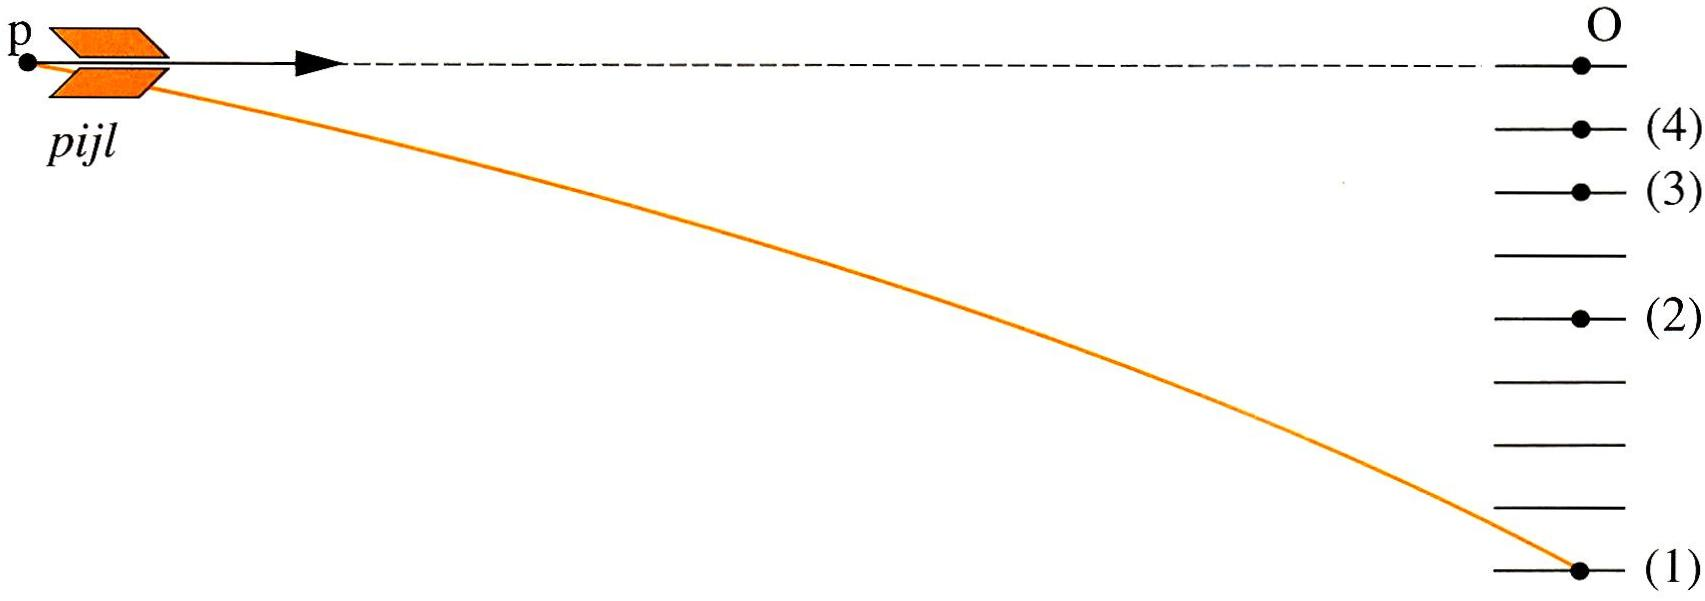
\includegraphics[width=0.8\textwidth]{afgeschotenpijl.jpg}
\end{center}
%%\end{figure}
\begin{oplossing}
We gebruiken de baanvergelijking van de
horizontale worp. Voor eenzelfde horizontale afstand $x$ moeten we
immers een nieuwe verticale afstand $y$ vinden, in functie van een
andere beginsneleheid. Als het accent ' staat voor de nieuwe
situatie waarin de beginsnelheid is verdubbeld, dan geldt:
\begin{eqnarray*}
y'&=&\frac{g}{2v_0'^2}x^2\\
&=&\frac{g}{2(2v_0)^2}x^2\\
&=&\frac{1}{4}\frac{g}{2v_0^2}x^2\\
&=&\frac{1}{4}y
\end{eqnarray*}
De pijl zal dus in punt (3) terechtkomen.
\end{oplossing}

\end{exercise}

\begin{exercise} Een puntmassa beschrijft een cirkel met een straal van $5,0\rm\,cm$ en een periode van $0,33\rm\,s$. Welke afstand op de cirkel legt deze puntmassa in $7,0\rm\,s$ af?
\begin{oplossing}
\textit{gevraagd}  $s$ (booglengte)

\textit{oplossing} Omdat de grootte van de snelheid constant is, is de
afgelegde weg over de boog gelijk aan de snelheid vermenigvuldigd met de tijd:
\begin{eqnarray*}
s&=&vt\\
&=&r\omega t\\
&=&\frac{2\pi r}{T}t\\
&=&6,7\rm\,m
\end{eqnarray*}
\end{oplossing}
\begin{oplossing}
$l=vt=r\omega t=\frac{2\pi r}{T}t=70\pi/33=6,66\rm\,m$
\end{oplossing}



\end{exercise}

\begin{exercise}[Opgave] Bereken de hoeksnelheid van de aarde om haar as. Bereken de
snelheid van een punt van het aardoppervlak:
\begin{enumerate}
\item aan de evenaar
\item op $51^\circ$ noorderbreedte.
\end{enumerate}
\begin{oplossing}
De hoeksnelheid kunnen we berekenen met de periode van de omwenteling van de aarde, nl. 24 uur, t.t.z. $86400\rm\,s$. Dat geeft
\begin{eqnarray*}
\omega=\frac{2\pi}{T}=\frac{2\pi}{86400\rm\,s}=7,3\cdot10^{-5}\rm\,rad\,s^{-1}
\end{eqnarray*}
De snelheid van een punt op het aardoppvlak aan de evenaar vinden we met het formuletje $v=r\omega$, waarbij $r$ de straal van de aarde\footnote{De straal van de aarde bedraagt 6370\rm\,km.} is.
\begin{eqnarray*}
v=r_a\omega=\frac{2\pi r_a}{T}=463\rm\,m/s
\end{eqnarray*}
Dit is nogal snel, het is namelijk $1667\rm\,km/h$. 
% \newline

Op $51^\circ$ noorderbreedte\footnote{Onze school ligt op $50^\circ 52'36,69"$ noorderbreedte.} maken we ook een cirkelbeweging maar nu met een andere straal. De straal is nu de afstand van het punt op het aardoppervlak tot aan de rotatieas van de aarde, zie figuur. 
%%\begin{figure}[h]
\centering
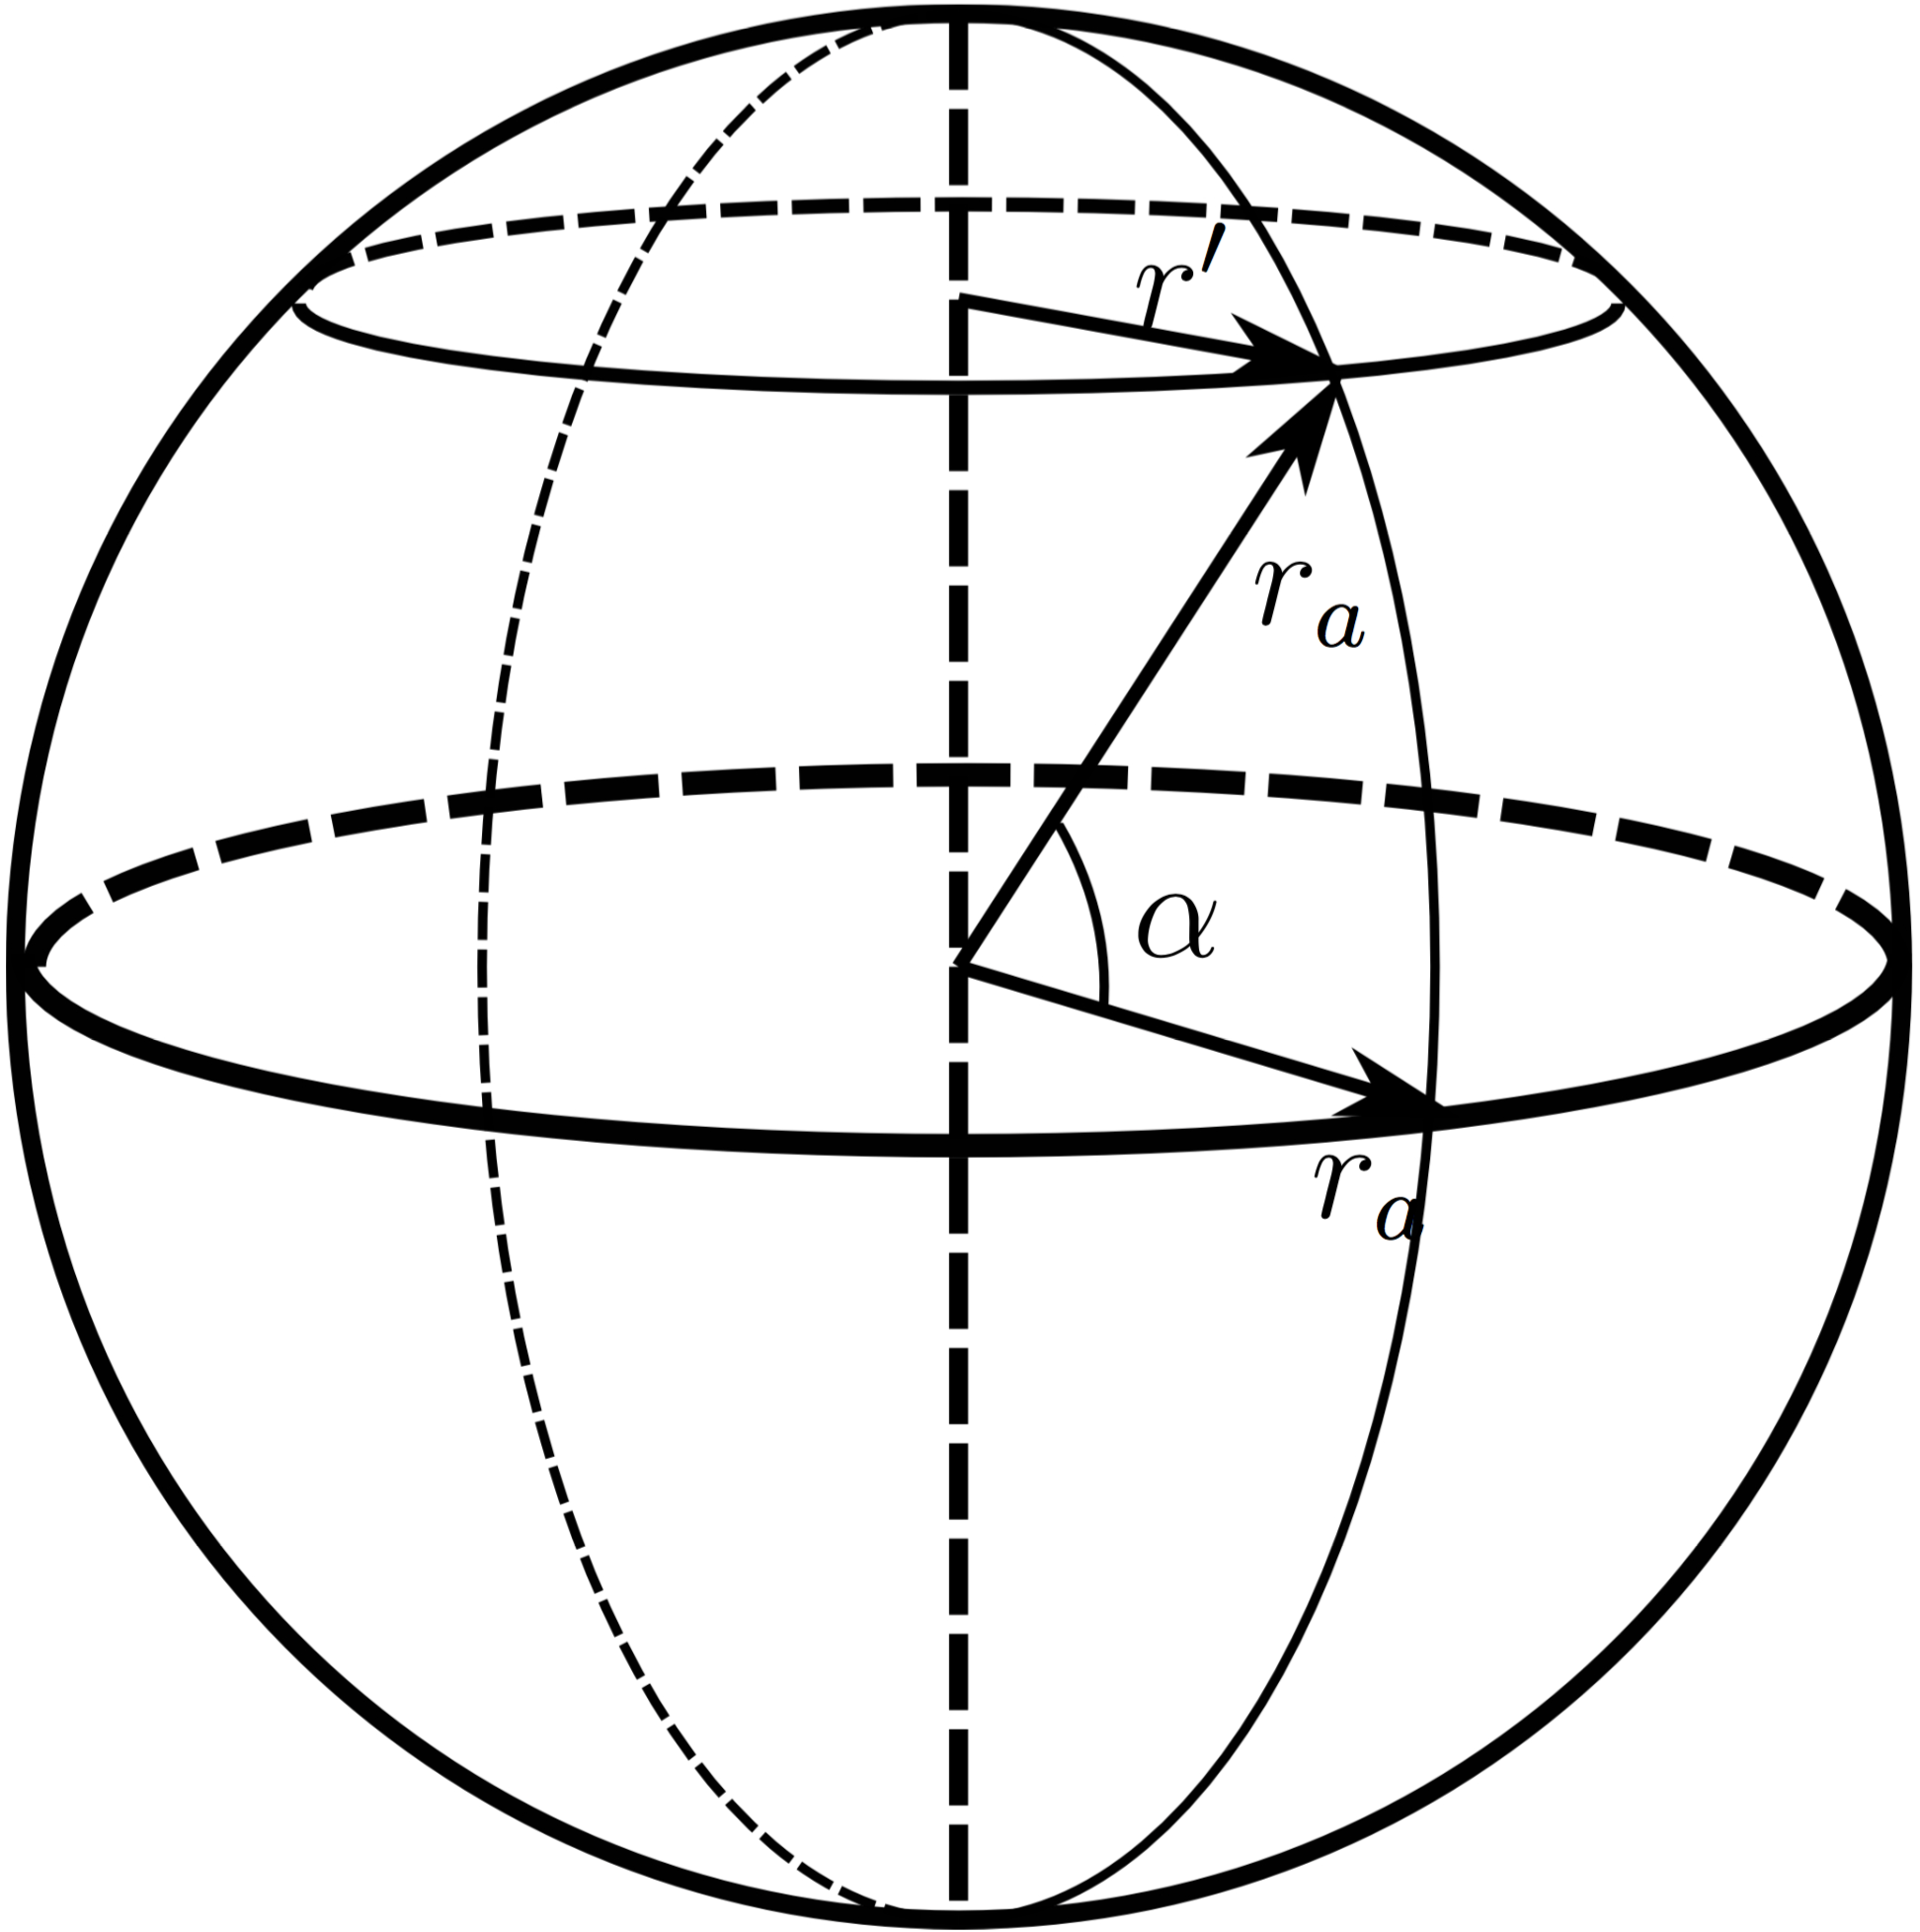
\includegraphics[width=0.4\textwidth]{aardehoeksnelheid2}
%%\end{figure}
%%%\begin{figure}[H]
%\begin{picture}(320,160)(0,0)
%\put(115,0){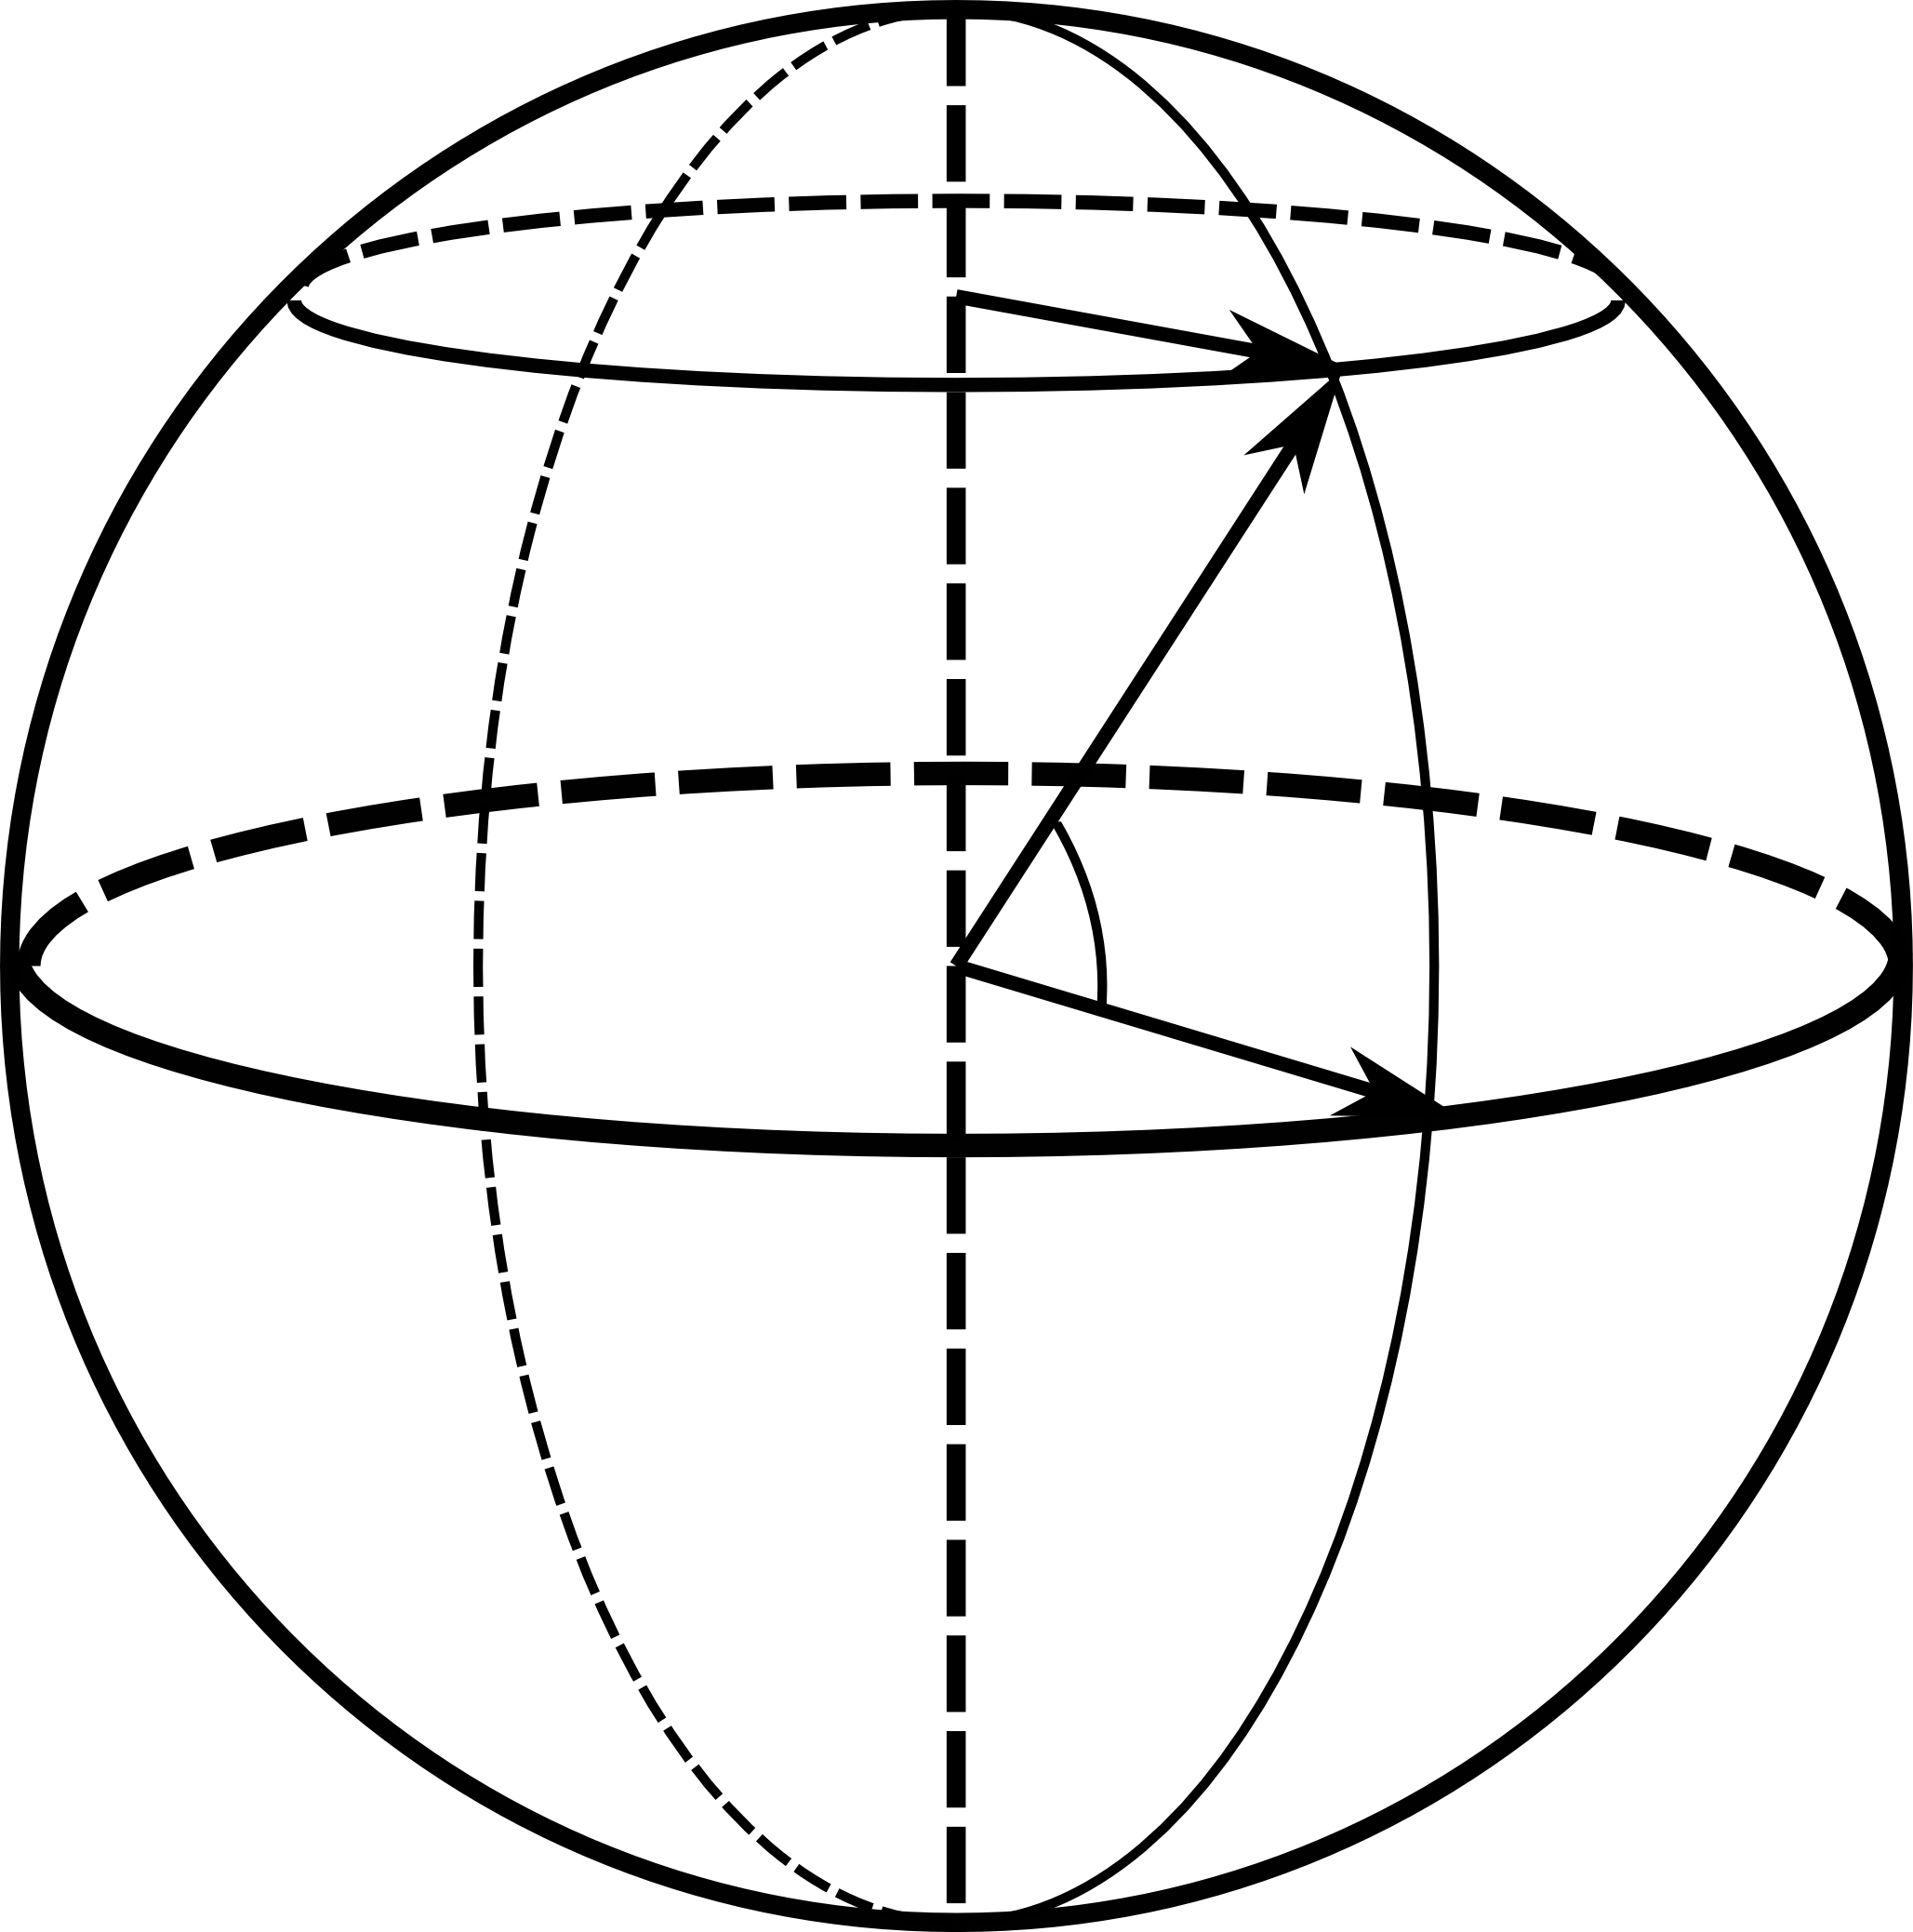
\includegraphics[scale=1.0]{aardehoeksnelheid}}
%\put(210,82){$\alpha$}
%\put(225,60){$r_a$}
%\put(220,110){$r_a$}
%\put(210,135){$r'$}
%%\put(0,0){bl}
%%\put(0,160){tl}
%%\put(390,0){br}
%%\put(390,160){.}
%\end{picture}
%%%\end{figure}
Met elementaire driehoeksmeetkunde vind je deze straal terug als $r'=r\cos\alpha$. De snelheid vinden we vervolgens op dezelfde manier.
\begin{eqnarray*}
v=r'\omega=\frac{2\pi r\cos\alpha}{T}=291\rm\,m/s
\end{eqnarray*}
Dit is ook nog snel, nl. $1048\rm\,km/h$.
\end{oplossing}



\end{exercise}

\begin{exercise} Een auto rijdt door een bocht met een constante snelheid van \SI{50}{km/h}. Heef de auto een andere versnelling wanneer hij diezelfde bocht neemt met een constante snelheid van \SI{70}{km/h}? Licht je antwoord toe.

\end{exercise}

\begin{exercise} Als een auto met \SI{60}{km/h} een scherpe bocht neemt, en daarna met dezelfde snelheid een flauwe bocht, is de versnelling dan in beide gevallen gelijk? Leg uit.

\end{exercise}

\begin{exercise} Tijdens het trainen van een ruimtevaarder wordt deze in een cir\-kel\-vor\-mi\-ge beweging gebracht met een zetel, die zich aan het uiteinde van een ho\-ri\-zon\-tale arm van $5,00\rm\,m$ lengte bevindt. Indien hij versnellingen tot $10g$ kan verdragen, wat is dan de toegelaten maximale snelheid, en het maximale toegelaten toerental?


\end{exercise}

\begin{exercise} 
\begin{minipage}[t]{0.5\textwidth}
Alle punten van een ring voeren een eenparige cirkelbeweging
uit. De grootte van de snelheid in punt A is $v_a$ en in punt B,
$v_b$. Dan is
\begin{enumerate}
\item $v_ar_a=v_br_b$
\item $v_br_a=v_ar_b$
\item $v_av_b=r_ar_b$
\item $v_a=v_b$
\end{enumerate}
\end{minipage}
\hspace{0.1\textwidth}
\begin{minipage}[t]{0.3\textwidth}
\raisebox{-5cm}{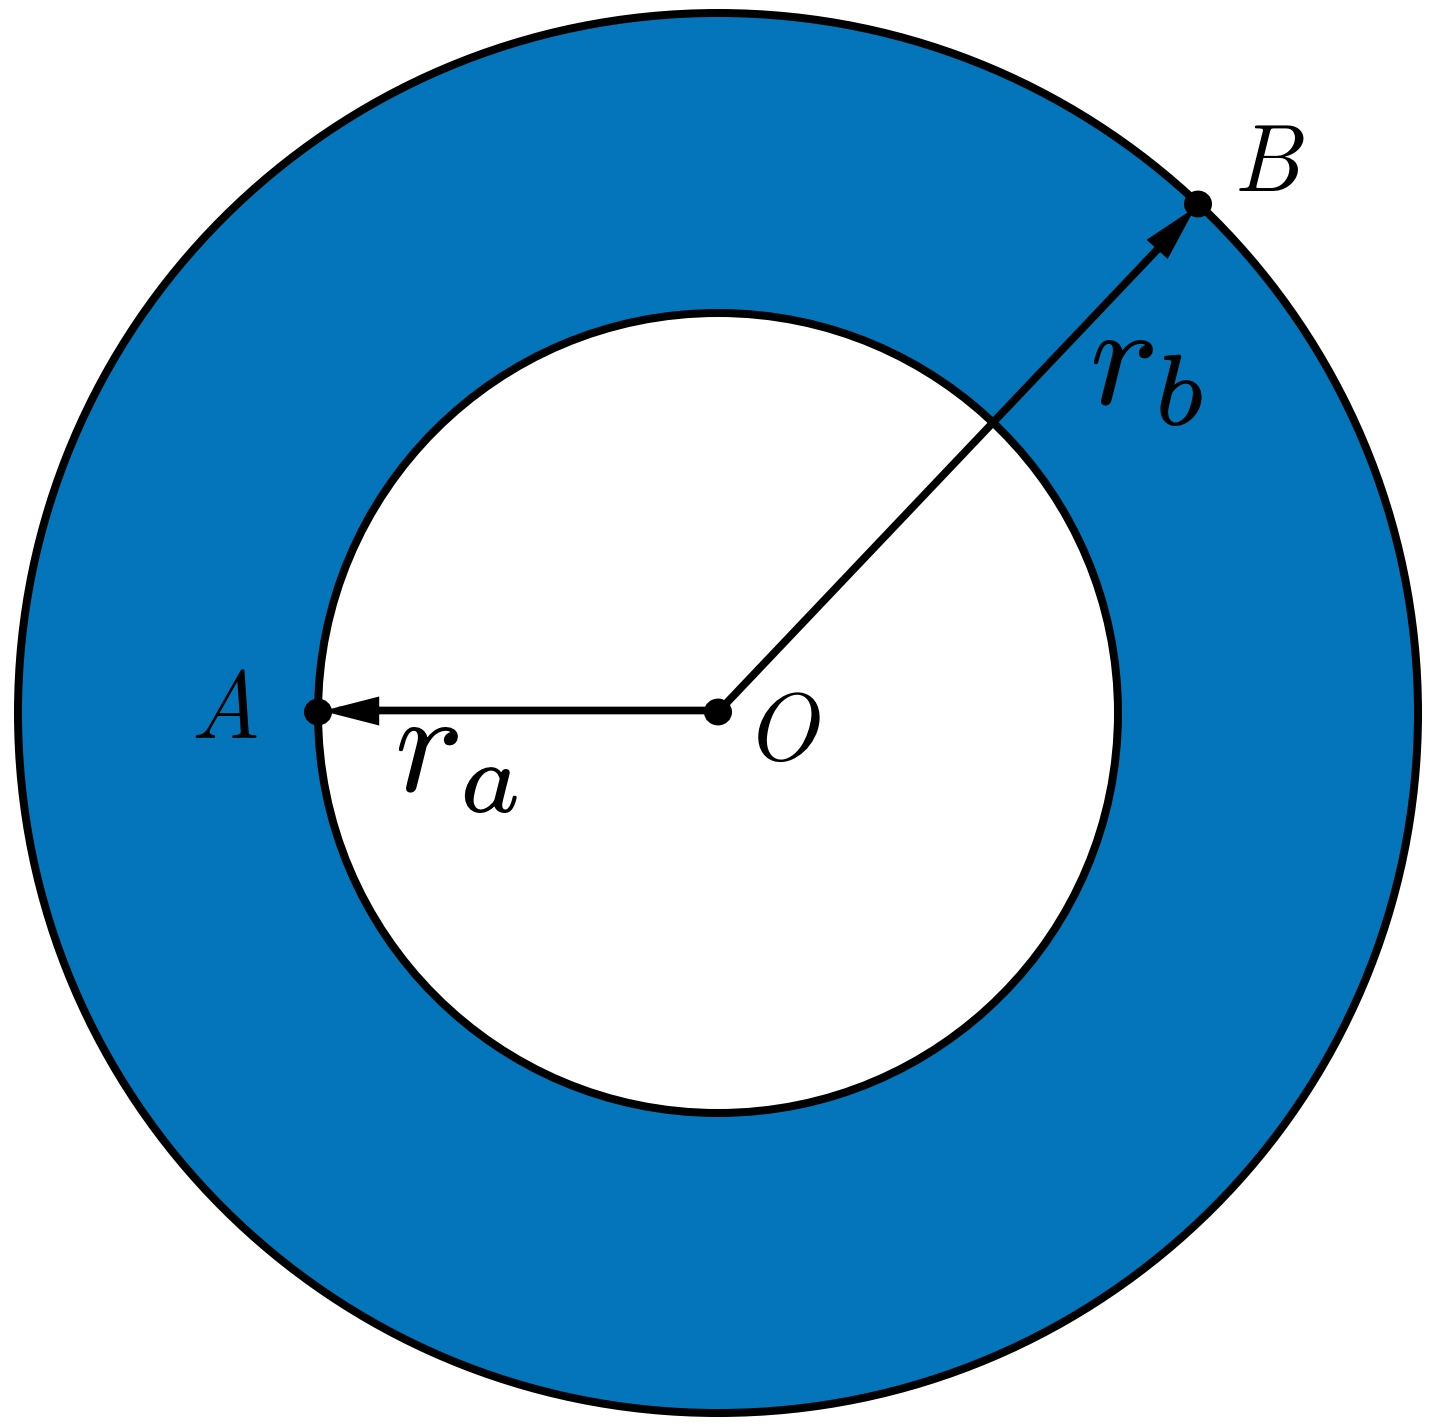
\includegraphics[width=\textwidth]{ringpunten}}
\end{minipage}
\begin{oplossing}
De hoeksnelheid is voor beide punten gelijk
zodat:
\begin{eqnarray*}
\omega_a&=&\omega_b\\
&\Updownarrow&\\
\frac{v_a}{r_a}&=&\frac{v_b}{r_b}\\
&\Updownarrow&\\
v_br_a&=&v_ar_b
\end{eqnarray*}
Het juist antwoord is dus (b).
\end{oplossing}

\end{exercise}

\begin{exercise} Bij een fiets zijn het grootste en het kleinste kamwiel door
middel van een ketting met elkaar verbonden. Tussen de hoeksnelheid
$\omega_1$ van het grootste kamwiel en $\omega_2$ van het kleinste
kamwiel bestaat de volgende relatie:
% \newline
\begin{minipage}[t]{0.4\textwidth}
\begin{enumerate}
\item $\omega_1=\omega_2$
\item $r_1\omega_2=r_2\omega_1$
\item $r_1\omega_1=r_2\omega_2$
\item $r_1r_2=\omega_1\omega_2$
\end{enumerate}
\end{minipage}
%\hspace{0.1\textwidth}
\begin{minipage}[t]{0.5\textwidth}
\raisebox{-3.5cm}{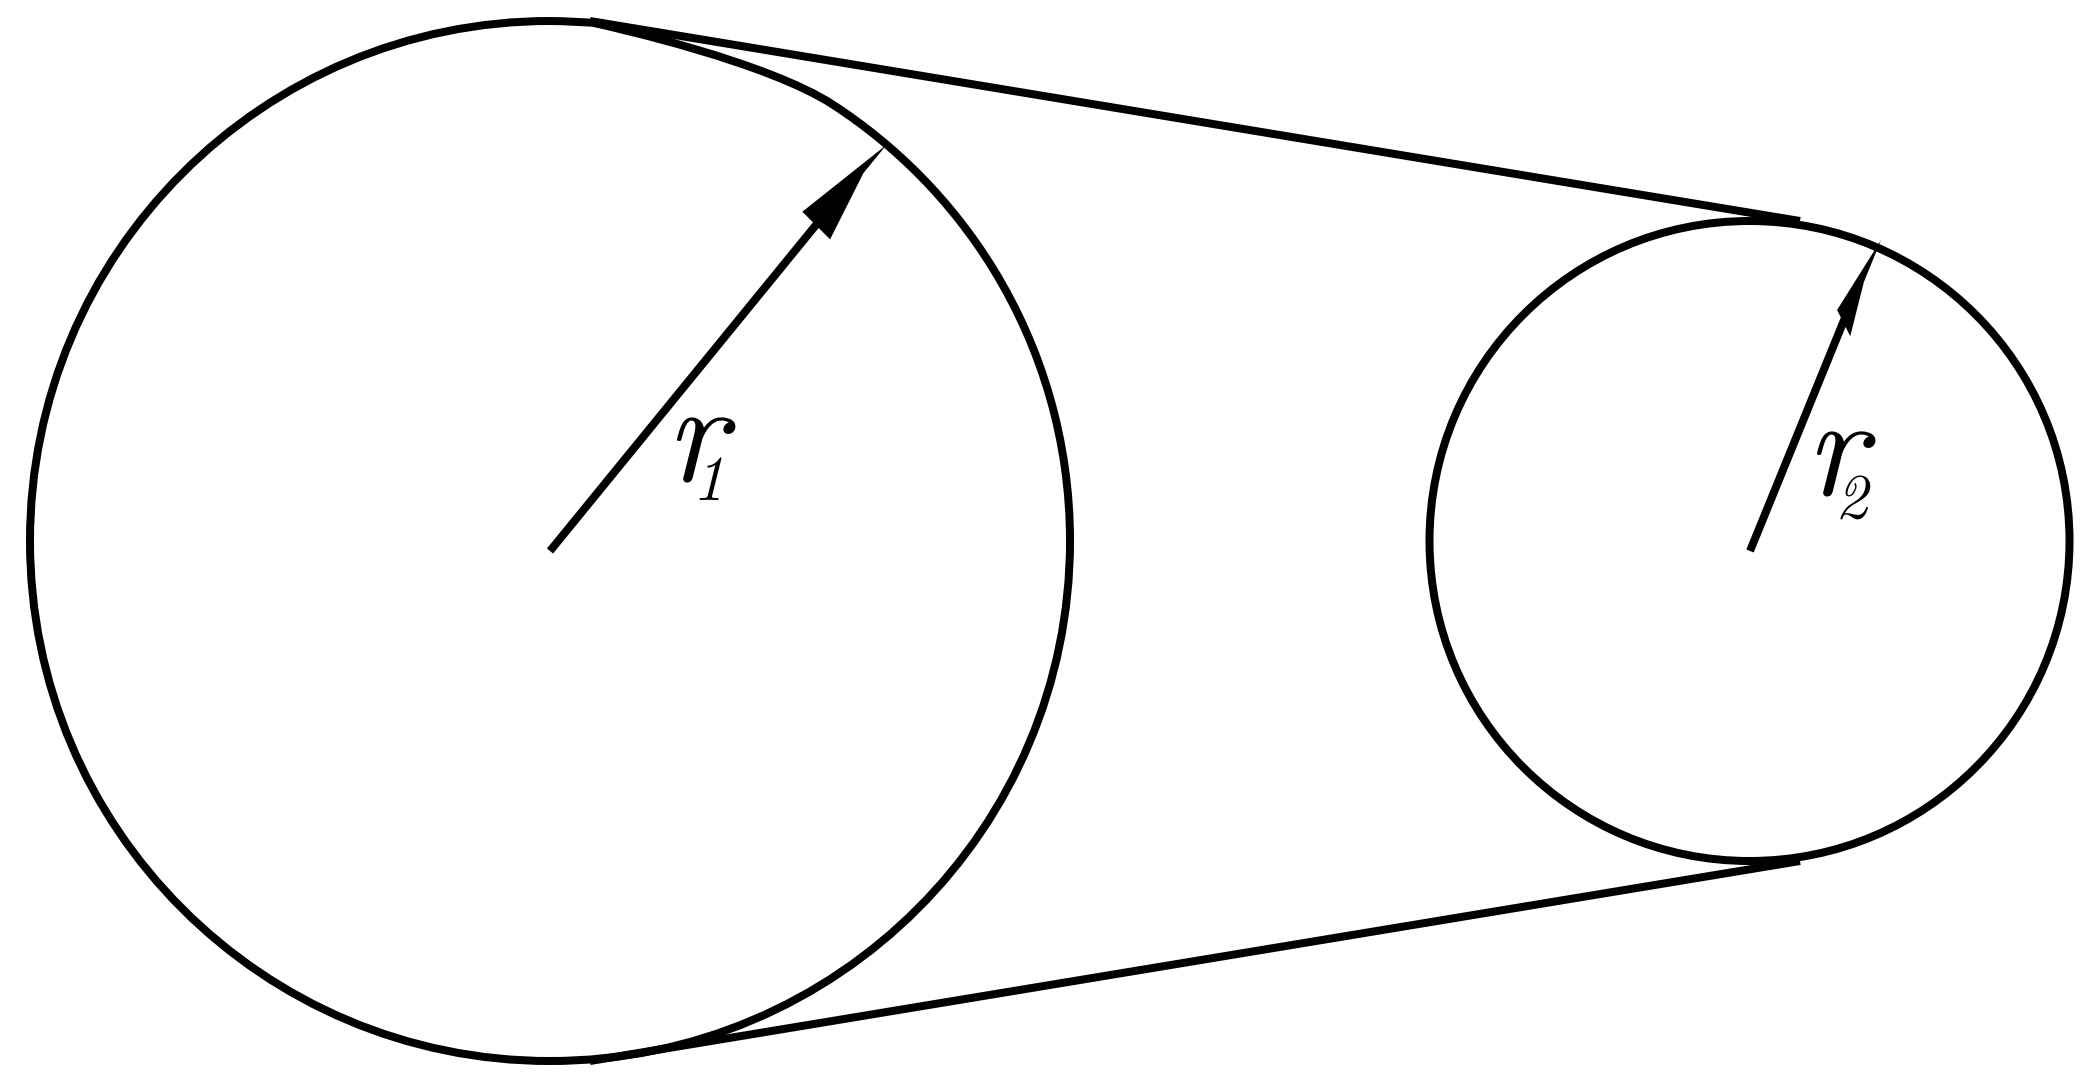
\includegraphics[width=\textwidth]{kamwielenfiets}}
\end{minipage}
\begin{oplossing}
Aangezien een stukje van de ketting overal
dezelfde snelheid heeft -- het legt in een bepaalde tijd steeds
evenveel afstand af -- moet de snelheid van een punt op de
buitenrand van het grootste wiel gelijk zijn aan de snelheid van een
punt op de buitenrand van het kleinste wiel. Dus:
\begin{eqnarray*}
v_1&=&v_2\\
&\Updownarrow&\\
r_1\omega_1&=&r_2\omega_2
\end{eqnarray*}
Het juist antwoord is dus (c).
\end{oplossing}



\end{exercise}

\begin{exercise} Een auto rijdt door een brugleuning en komt $5,2\rm\,m$ lager in het water terecht. De horizontale afstand tussen de plaats waar hij door de leuning ging en waar hij in het water terechtkwam, is $22\rm\,m$. Kan de politie hieruit afleiden met welke snelheid hij ongeveer reed? Was zijn werkelijke snelheid groter of kleiner?
\begin{oplossing}
\begin{eqnarray*}
y&=&\frac{g}{2v_0^2}x^2\\
&\Updownarrow&\\
v_0&=&x\sqrt{\frac{g}{2y}}=21,37\rm\,m/s=77\rm\,km/h
\end{eqnarray*}
\end{oplossing}



\end{exercise}

\begin{exercise}[Opgave] Een vliegtuig vliegt met een snelheid van $450\rm\,km/h$ op een hoogte van $920\rm\,m$.
\begin{enumerate}
\item Hoever voor het doel moeten de voedselpakketten gelost worden om op het doel terecht te komen?
\item Hoeveel tijd hebben de pakketten nodig om het doel te bereiken?
\end{enumerate}
\begin{oplossing}
\textit{gegeven}  $v_0=125\rm\,m/s$\newline$y=920\rm\,m$

\textit{gevraagd} $x$, $t$

\textit{oplossing} De afstand waarover de voedselpakketten in
horizontale richting zijn vooruit gegaan, kunnen we vinden met de
baanvergelijking. We weten namelijk hoever de pakketten naar beneden
zijn gevallen en wat hun beginsnelheid is:
\begin{eqnarray*}
y&=&\frac{g}{2v_0^2}x^2\\
&\Downarrow&\\
x&=&v_0\sqrt{\frac{2y}{g}}=1712\rm\,m
\end{eqnarray*}
De valtijd voor de pakketten vinden we o.a. door naar de verticale
valbeweging te kijken. Deze gebeurt onafhankelijk van wat er in de
horizontale richting gebeurt, zodat:
\begin{eqnarray*}
y&=&\frac{1}{2}gt^2\\
&\Downarrow&\\
t&=&\sqrt{\frac{2y}{g}}=13,7\rm\,s
\end{eqnarray*}
\end{oplossing}









\end{exercise}

\begin{exercise} Een vliegwiel doet 450 omwentelingen per minuut. Zoek de hoeksnelheid van het wiel en de snelheid van een punt op $1,70\rm\,m$ van het middelpunt.

\end{exercise}

\begin{exercise} In een bocht met straal $160~\rm m$ verlaagt een autorenner
zijn snelheid eenparig van $90~\rm m/s$ tot $75~\rm m/s$ in $2~\rm
s$. Bereken de grootte van de versnelling van de wagen op het
ogenblik dat de snelheid $80~\rm m/s$ is.
\begin{enumerate}
\item $40,7~\rm m/s^2$
\item $40~\rm m/s^2$
\item $15~\rm m/s^2$
\item $7,5~\rm m/s^2$
\end{enumerate}
\footnote{(antw. b)}

\end{exercise}

\begin{exercise} In de figuur is de versnelling en de snelheid van een puntmassa gegeven op een bepaald tijdstip. De grootte van de versnelling is $15,0\rm\,m/s^2$ en de vector maakt een hoek van $30^\circ$ met de straal van de cirkel. De straal van de cirkel is $2,50\rm\,m$. Bepaal de grootte van de normaalversnelling, de grootte van de tangenti\"ele versnelling en de grootte van de baansnelheid.
%ECB_tangentieel nog invoegen ... !




\cleardoublepage

\section{Schuine worp}

\end{exercise}

\begin{exercise} Leid een formule af die bij een schuine worp de dracht
(draagwijdte) geeft in functie van de beginsnelheid en de hoek
waaronder wordt geschoten.

\end{exercise}

\begin{exercise} Een projectiel wordt met een beginsnelheid van $350\rm\,m/s$
onder een hoek van $30^\circ$ met de horizontale afgeschoten.
\begin{enumerate}
\item Welke hoogte bereikt het projectiel?
\item Waar komt het projectiel op de grond?
\end{enumerate}
\footnote{$h=1561\rm\,m$, $d=10814\rm\,m$}

\end{exercise}

\begin{exercise} Een puntmassa wordt met een beginsnelheid van $40\rm\,m/s$
onder een hoek van $60^{\circ}$ opgeworpen.
\begin{enumerate}
\item Hoe groot is de snelheid in een punt op $35\rm\,m$ hoogte?
\item Hoe groot is de hoek, die de snelheid met de horizontale maakt in een punt
op $35\rm\,m$ hoogte boven de grond?
\item Waaraan is deze hoek gelijk als het voorwerp weer op dezelfde
hoogte is maar bij de dalende beweging?
\item Onder welke hoek treft het voorwerp de grond?
\end{enumerate}

\end{exercise}

\begin{exercise} Een obus wordt met een beginsnelheid $\vec{v}_0$ en onder een
hoek $\varphi$ weggeschoten. In het hoogste punt van zijn baan is:
\begin{enumerate}
\item $v_x=0\rm\,m/s$;
\item $v_x=h/t$;
\item $v_x=v_y$;
\item $v_x=v_0\cos{\varphi}$.
\end{enumerate}
\footnote{antwoord d}

\end{exercise}

\begin{exercise} Verschillende tennisballen worden met even grote snelheid maar
onder een verschillende hoek weggeschoten. De tennisbal die de
grootste dracht bereikt is deze die weggeschoten wordt onder een
hoek van:
\begin{enumerate}
\item 22,5$^\circ$;
\item 45,0$^\circ$;
\item 67,5$^\circ$;
\item 90,0$^\circ$.
\end{enumerate}
\footnote{antwoord b}

\end{exercise}

\begin{exercise} Twee raketten worden vanuit eenzelfde punt schuin
weggeschoten. Hun beginsnelheid is even groot en hun beginhoeken
zijn complementair ($\alpha+\beta=\frac{\pi}{2}$). Hebben deze
raketten dezelfde dracht?

\end{exercise}

\begin{exercise} Vanop de top van een kerktoren van $75,0\rm\,m$ hoog schiet
men een projectiel onder een hoek van $40^\circ$ met de horizontale
weg. De grootte van de beginsnelheid is $400\rm\,m/s$. Na hoeveel
tijd bereikt het projectiel de grond, en op welke afstand van de
voet van de toren? \footnote{$t=52,7\rm\,s$, $x=16151\rm\,m$}

\end{exercise}

\begin{exercise} Toon met een volledige opbouw aan dat de formule voor de
maximale hoogte bij de schuine worp wordt gegeven door:
\begin{displaymath}
h=\frac{v_0^2\sin^2{\varphi}}{2g}
\end{displaymath}

\end{exercise}

\begin{exercise} Een projectiel wordt afgevuurd met een beginsnelheid
$\vec{v}_0$ die een hoek $\varphi$ maakt met de horizontale
\mbox{$x$-as}.
% \newline
In de veronderstelling dat de luchtweerstand verwaarloosbaar is, dan
ziet het verloop van de horizontale snelheidscomponente $v_x$ als
functie van de tijd er als volgt uit:
%%\begin{figure}[h]
\begin{flushright}
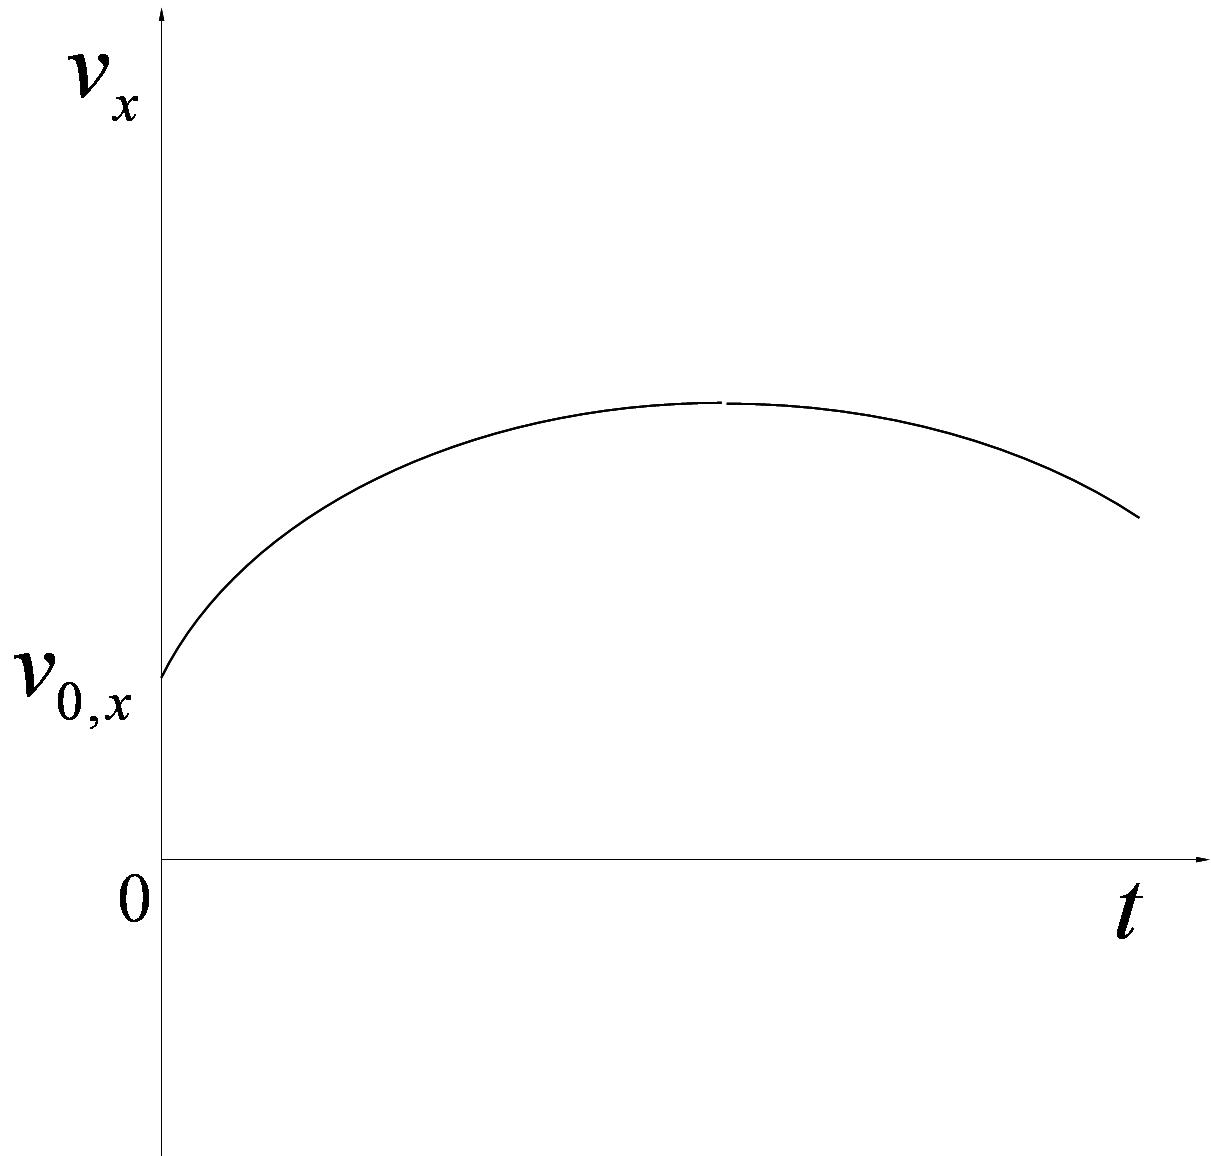
\includegraphics[width=0.22\textwidth, angle=0]{horiz_snelheidscomp_a}
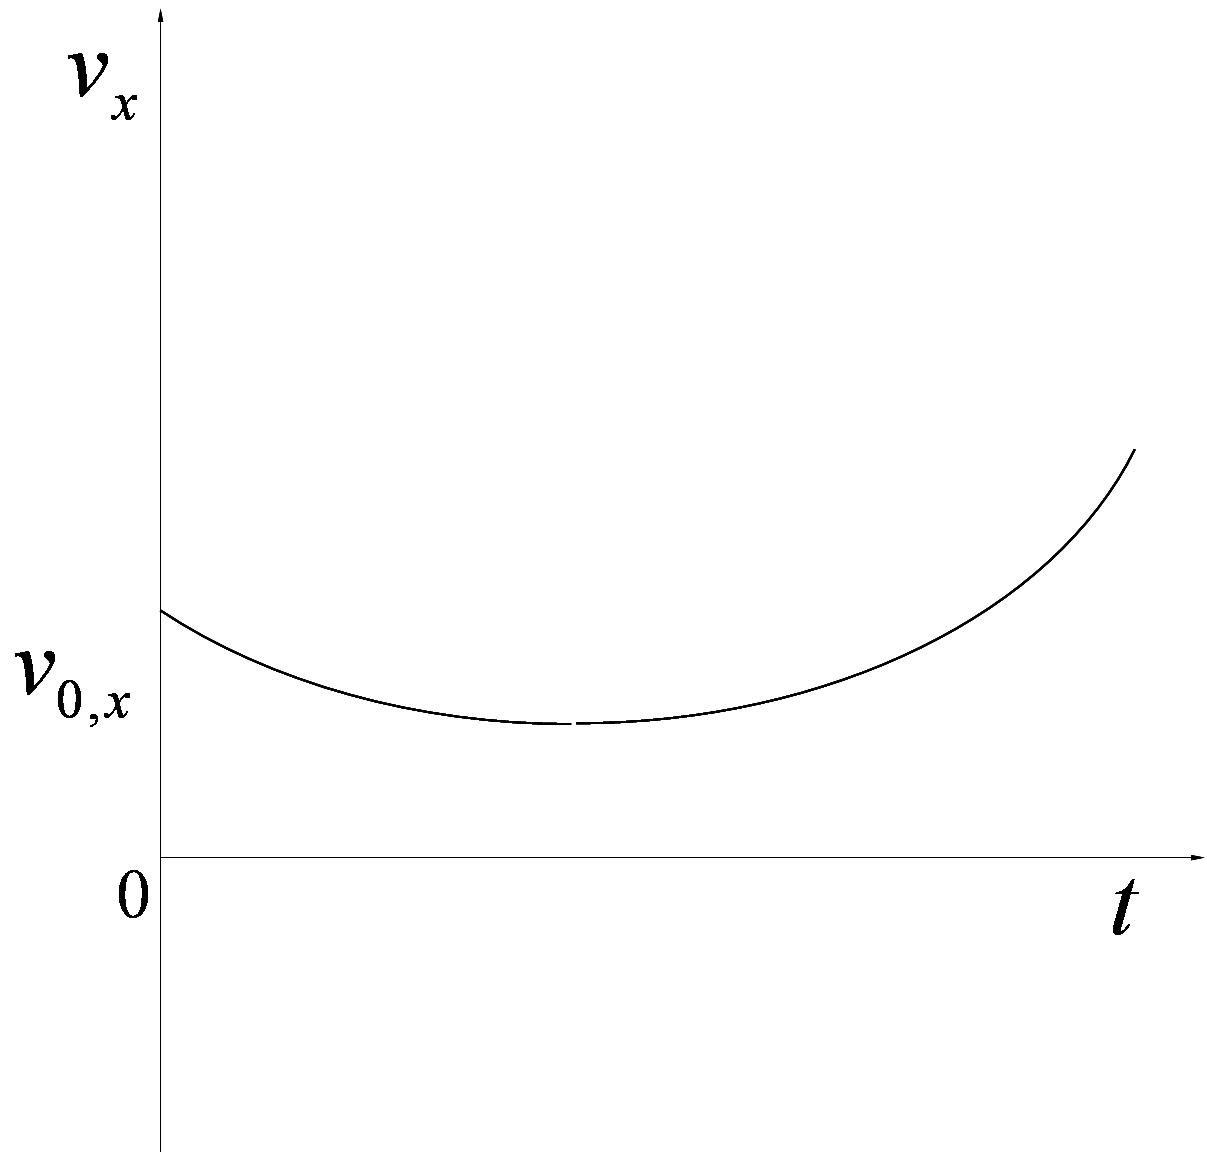
\includegraphics[width=0.22\textwidth, angle=0]{horiz_snelheidscomp_b}
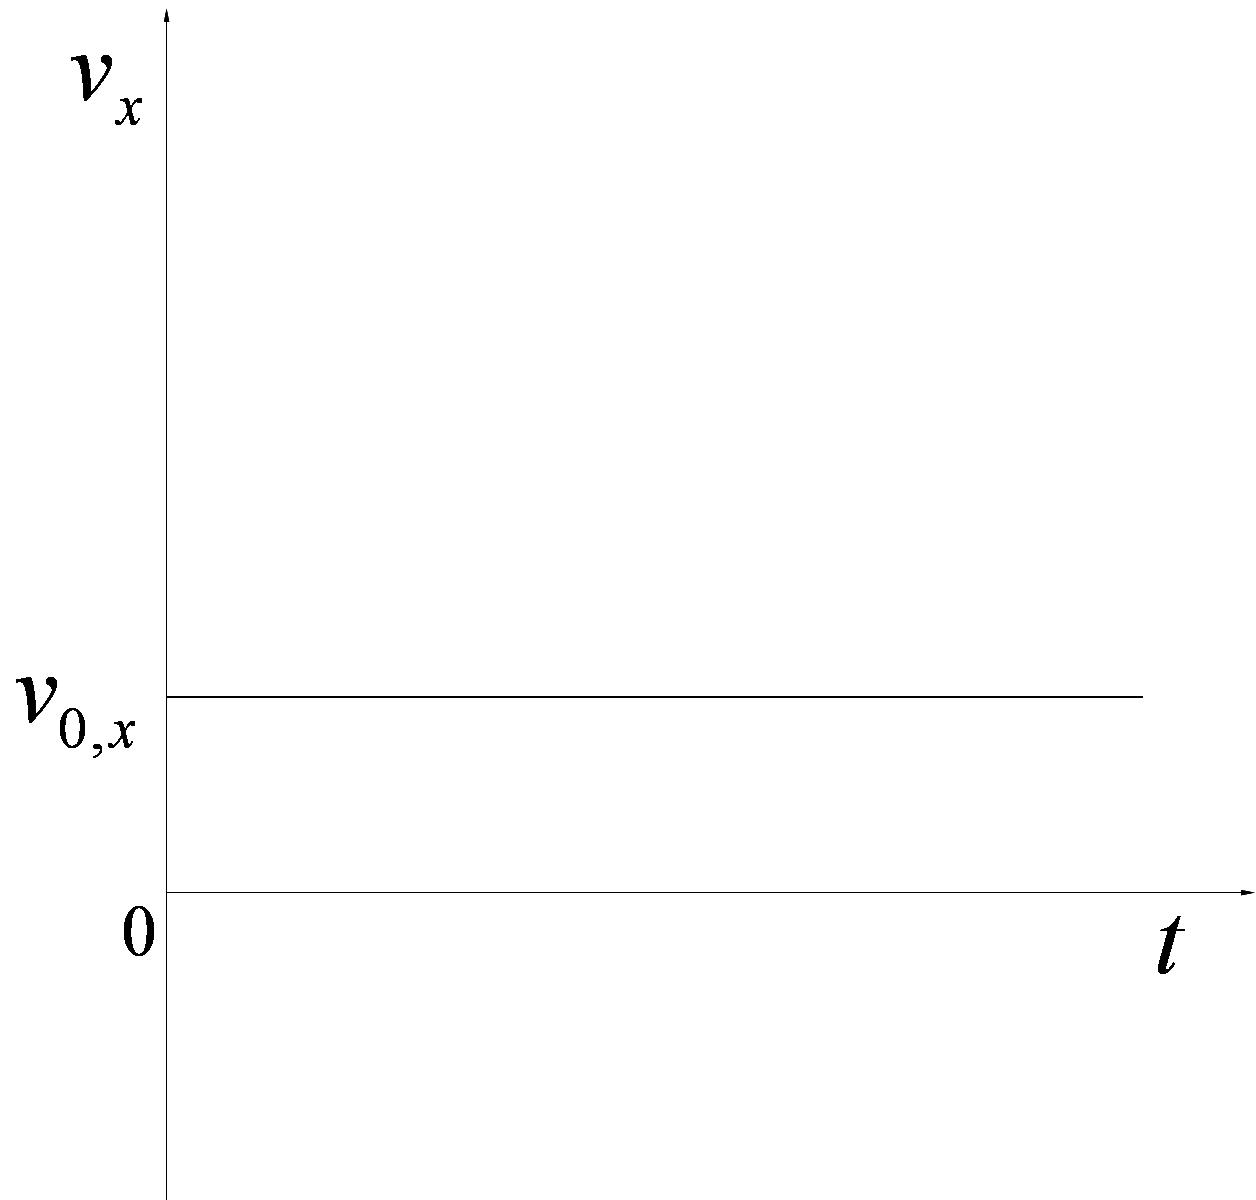
\includegraphics[width=0.22\textwidth, angle=0]{horiz_snelheidscomp_c}
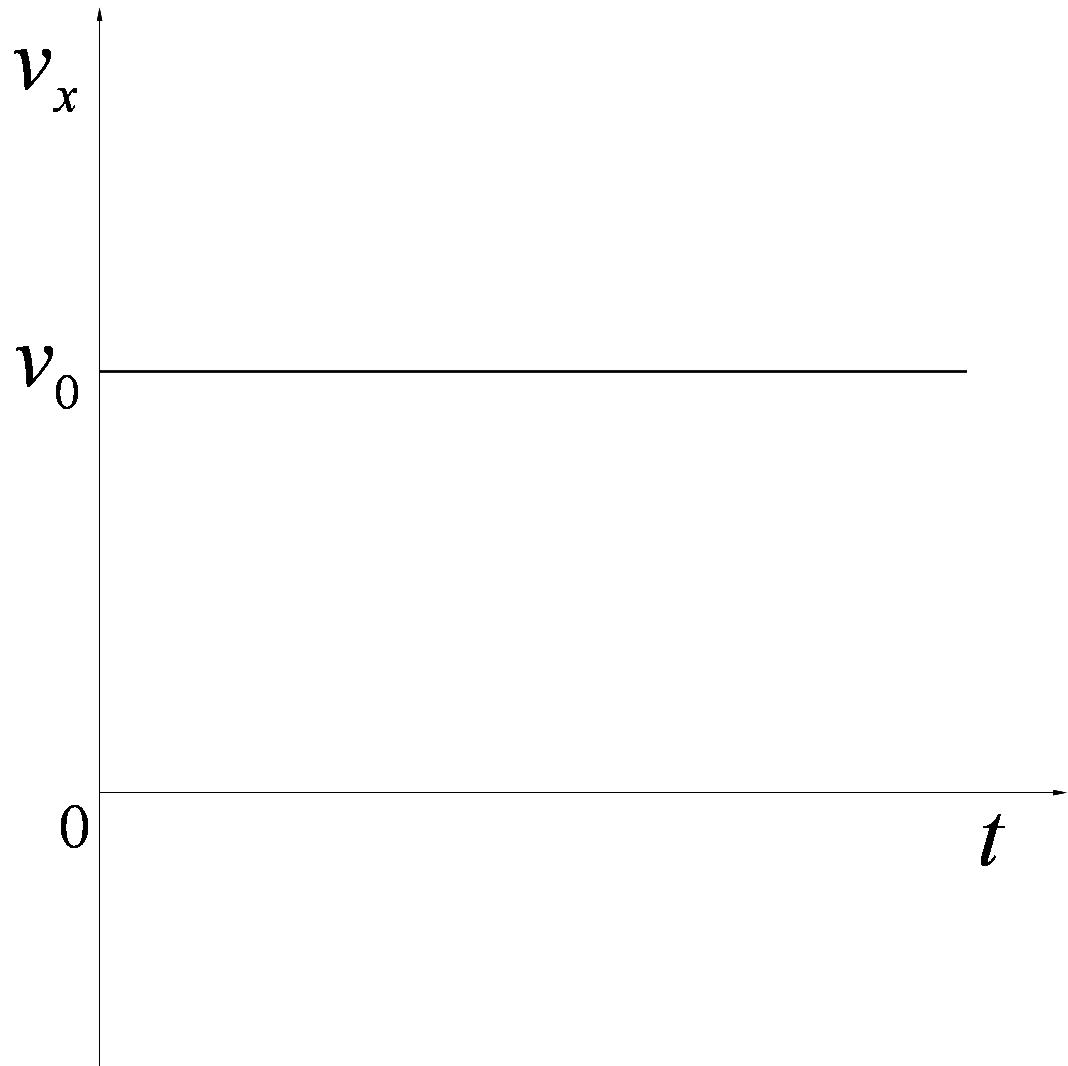
\includegraphics[width=0.22\textwidth, angle=0]{horiz_snelheidscomp_d}
\end{flushright}
%%\end{figure}

\end{exercise}

\begin{exercise} Onderstaande figuur stelt de baan voor van
een kogel die op het ogenblik \mbox{$t=0$~s} afgeschoten wordt
vanuit de oorsprong. De aangeduide punten geven om de \mbox{100 ms}
de plaats van de kogel aan.
%%\begin{figure}[h]
\begin{center}
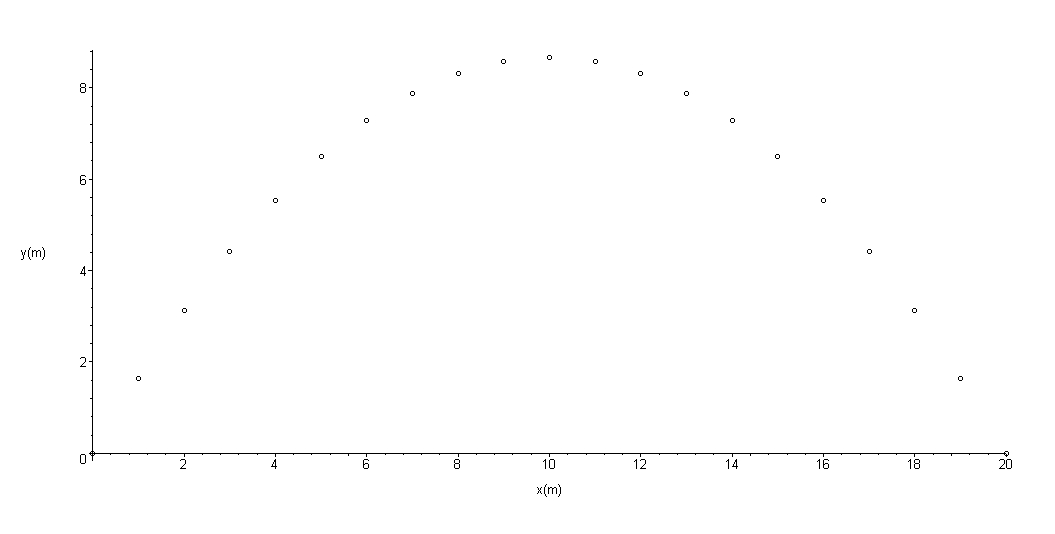
\includegraphics[width=0.7\textwidth]{horiz_snelheidscomp}
\end{center}
%%\end{figure}


De horizontale snelheidscomponent van de kogel is gelijk aan?
\begin{enumerate}
\item 5 m/s
\item 10 m/s
\item 15 m/s
\item 20 m/s
\end{enumerate}

\end{exercise}

\begin{exercise} Nadat de kerstman zijn speelgoed op de
gebruikelijke manier geleverd heeft, wil hij zich ook eens amuseren
en glijdt langs het beijzeld dak naar beneden. Hij vertrekt vanuit
rust op de top van het dak dat $8,2~\rm m$ lang is met een
versnelling van $5,0~\rm m/s^2$. De rand van het dak bevindt zich
$3,0~\rm m$ boven de grond die met een pak sneeuw bedekt is.
%%\begin{figure}[h]
\begin{center}
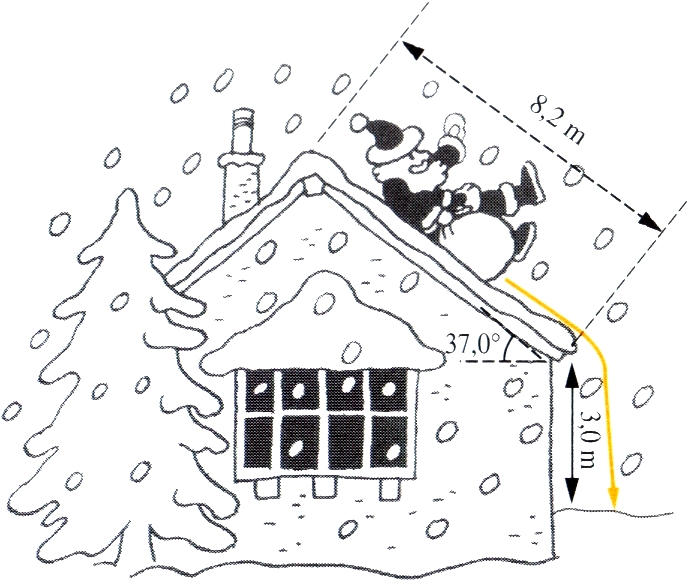
\includegraphics[width=0.55\textwidth]{kerstman}
\end{center}
%%\end{figure}
\begin{enumerate}
\item Hoe groot is de snelheid van de kerstman waarmee hij van het
dak vliegt?
\item Hoe groot is de afstand $d$ tussen het huis en het punt waar
hij in de sneeuw terecht komt?\footnote{De baanvergelijking voor de
schuine worp:
\[
y=x\tan\varphi-\frac{g}{2v_0^2\cos^2\varphi}x^2
\]}
\end{enumerate}

\end{exercise}


\end{document}